% ================================================
% =                INTRODUCTION                  =
% ================================================ 
The development of \aclink{ADS} has been a hot topic in the automotive industry for the last years. These systems rely on a combination of sensors and algorithms to perform driving tasks, either partially or fully replacing the human driver. A fundamental component of any ADS is its perception system,  which is responsible for detecting obstacles and generating a reliable representation of the surrounding environment.

One key element within the perception system is the generation of a local \aclink{BEV} map. A local \aclink{BEV} map provides a top-down, 2D representation of the vehicle's immediate surroundings, typically centered on the vehicle's position. Unlike raw sensor data, which is captured from the perspective of individual cameras or LiDAR units, the \aclink{BEV} map projects this information onto an unified ground-level plane, creating a structured grid in metric space. Each cell in the grid represents a precise location in the real world, enabling the system to interpret spatial relationships between road elements, obstacles, and free space with high accuracy.

Generating a segmented \aclink{BEV} map improves the perception system by providing rich semantic information and precise obstacle localization within a metric space. Semantic \aclink{BEV} representations are useful for a variety of tasks, including scene understanding, map reconstruction, behavior prediction of surrounding agents, and trajectory planning.

To obtain \aclink{BEV} semantic segmentation from cameras, traditional methods first generate semantic masks in image space and then transform them into \aclink{BEV} space using \aclink{IPM}. Despite its simplicity, it requires accurate camera parameters and assumes a perfectly flat ground surface, which limits its effectiveness. Moreover, while planar or low-height objects such as road curbs, lane markings, and the drivable area retain a meaningful metric representation in \aclink{BEV} space, objects with height appear distorted after the transformation.

With the objective of addressing the afore mentioned limitations, recent methods leverage data-driven techniques for \aclink{BEV} representation \cite{view_parsing_network} \cite{lift_splat_shoot} \cite{m2bev}. However, to the best of our knowledge, no prior work has investigated the impact of training a standard semantic segmentation model directly on \aclink{BEV} images, with the aim of evaluating whether this approach improves performance on planar elements.

The main objective of this master's thesis is to investigate the hypothesis: \textit{Does training a semantic segmentation model directly on \aclink{BEV} images outperforms the traditional image-space segmentation followed by \aclink{IPM} reprojection?} Additionally, this work explores a technical application of \aclink{BEV} semantic segmentation for annotating vehicular scenes with occupancy, occlusion, and drivable area masks, contributing to the field of monocular 3D object detection given 2D semantic masks.





% ================================================ 
% The development of \aclink{ADS} has been a hot topic in the automotive industry for the last years. One of the fundamental aspects of an \aclink{ADS} is the perception system, as it is responsible for performing the obstacle detection and to provide a good environment representation for other systems, among others. This perception system can be divided into two main tasks: 3D object detection and local \aclink{BEV} map generation. 
% 3D object detection is usually based on pointclouds obtained from \aclink{LiDAR} sensors, but as this sensors are costly a lot of research has been made in the field of camera 3D object detection. This approach has been gaining a lot of popularity carried by the improvements of the computer vision techniques with deep learning.
% \aclink{BEV} segmentation aims to create a semantic representation of a vehicle's surroundings. This is a key component of an \aclink{ADS} perception system as \aclink{BEV} segmentation provides rich semantic information, precise localization, and absolute scales. This makes it useful for various tasks, including map reconstruction, prediction of agent intentions, and vehicle path planning.
% To obtain \aclink{BEV} semantic segmentation from cameras, traditional methods first generate semantic masks in image space and then transform them into \aclink{BEV} space using \aclink{IPM}. Despite its simplicity, it requires accurate camera parameters and assumes a perfectly flat ground surface, which limits its effectiveness. Moreover, while planar or low-height objects such as road curbs, lane markings, and the drivable area retain a meaningful metric representation in \aclink{BEV} space, objects with height appear distorted after the transformation.
% With the objective of addressing the afore mentioned limitations, recent methods leverage data-driven techniques for \aclink{BEV} representation \cite{view_parsing_network} \cite{lift_splat_shoot} \cite{m2bev}. However, to the best of our knowledge, no previous work has explored training a standard semantic segmentation model directly on \aclink{BEV} images to measure the difference between the inference of planar elements.
% This master's thesis seeks to answer the question: \textit{Does a model directly trained on semantic BEV images outperforms a typical segmentation model for plannar elements?}. Additionally, this work explores a technical application of \aclink{BEV} semantic segmentation for annotating vehicular scenes with occupancy, occlusion, and drivable area masks, contributing to the field of monocular 3D object detection given 2D semantic masks.



% ================================================
% =                 OBJECTIVES                   =
% ================================================ 
\subsection{Objectives}
This master's thesis aims to address key challenges in \aclink{BEV} semantic segmentation. While initially motivated by the investigation of optimal BEV segmentation strategies, this work also explores a tangible real-world application of these techniques in the \aclink{ADS} context. Accordingly, it focuses on achieving two main objectives: to analyze semantic segmentation in \aclink{BEV} space for planar elements by comparing a traditional strategy with a proposed alternative approach (\textbf{O1}), and to implement an annotation system for generating BEV masks for occupancy, occlusion, and drivable areas (\textbf{O2}).

\begin{figure}[h!]
    \centering
    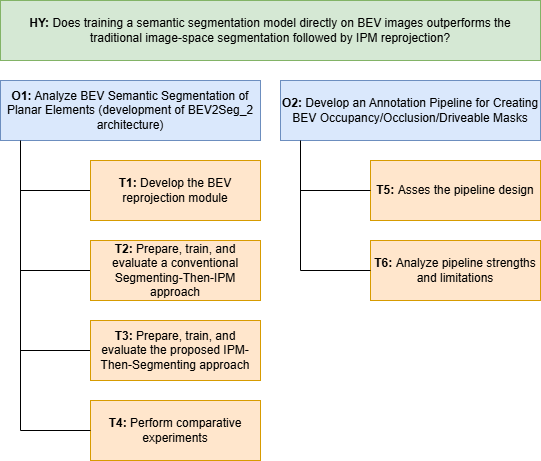
\includegraphics[width=0.8\linewidth]{./images/introduction/TFM_Objectives.png}
    \caption{Thesis objectives and tasks}
    \label{fig:objectives}
\end{figure}

To address the first objective, a methodology named BEV2Seg\_2 has been developed, establishing a common comparison framework between the classical image-space segmentation followed by \aclink{IPM} reprojection and the proposed direct \aclink{BEV} segmentation approach. Within this framework, a shared semantic segmentation model must be selected and adapted to both strategies to ensure consistency in the architecture design. The model will be trained under two different configurations: using conventional perspective images (\textbf{T2}), and using \aclink{BEV} reprojected images (\textbf{T3}). This dual training approach will produce two versions of the model architecture, each corresponding to one of the compared strategies.

To ensure a fair and valid comparison, the same original dataset will be used as the input source for both training pipelines. From this dataset, \aclink{BEV} reprojected images and their corresponding semantic masks will be generated to serve as training data for the proposed \aclink{BEV} based approach. Consequently, a common \aclink{BEV} reprojection module must be developed (\textbf{T1}). This module will apply consistent transformation parameters and serve two key purposes: generating the \aclink{BEV} training dataset and reprojecting inferenced results from the traditional strategy. In doing so, it ensures that both models are evaluated on an identical validation set composed of \aclink{BEV} semantic masks, thereby allowing for a reliable and unbiased performance comparison.

The second objective of this thesis involves developing a practical application of \aclink{BEV} semantic segmentation by implementing an automated annotation pipeline (\textbf{T5}). This pipeline aims to generate masks in \aclink{BEV} space that represent occupancy, occlusion, and drivable areas from vehicular scene data. This directly addresses the need for real-world utility of \aclink{BEV} semantic masks for downstream tasks such as motion planning and dynamic obstacle handling. Alongside the implementation, a critical analysis of the solution will be carried out to assess its effectiveness, strengths, and limitations (\textbf{T6}).

To achieve the stated objectives, this master's thesis relied on a diverse set of software tools and hardware resources for dataset generation, model training and validation, and annotation pipeline implementation. Python was the main programming language used for most of the custom implementations. Docker was extensively used for software packaging and environment consistency, facilitating interactions with a High-Performance Computing system for model training and enabling the creation of automated systems essential for annotation generation. Furthermore, various visualization tools such as WebLABEL and Open3D were employed to support development and analysis throughout the project.

This project was conducted over a seven-month period at Vicomtech  \footnote{\url{https://www.vicomtech.org/en/}}. Vicomtech, is a research center in applied Artificial Intelligence, VisualComputing, and Interaction which provided the necessary hardware infrastructure and technical support for this thesis.



% ================================================ 
% This master's thesis aims to address key challenges in \aclink{BEV} semantic segmentation and its practical applications within autonomous driving systems. While initially motivated by the investigation of optimal BEV segmentation strategies, this work also explores a tangible real-world application of these techniques.
% Respectively, the main objectives of this thesis are:
% \begin{enumerate}
%     \item \textbf{Evaluate \aclink{BEV} segmentation strategies performance for planar elements:} To empirically determine whether a semantic segmentation model directly trained on \aclink{BEV} images outperforms a traditional pipeline that involves segmentation in image space followed by \aclink{IPM} reprojection, specifically focusing on the segmentation of planar elements. In addressing this primary question, other crucial sub-questions are also investigated:
%         \begin{itemize}
%             \item \textbf{Asses label merging impact:} To evaluate if merging semantically similar labels during training can enhance model performance, parcularly for low-presence classes in \aclink{BEV} images.
%             \item \textbf{Identify effective data augmentation:} To determine which data augmentation techniques are most effective for training semantic segmentation models directly on \aclink{BEV} images.
%         \end{itemize}
%     \item \textbf{Develop a \aclink{BEV} scene annotation pipeline:} To implement a practical application of \aclink{BEV} semantic segmentation by creating an automated pipeline for generating occupancy, occlusion, and drivable area masks from vehicular scenes. This directly addresses the need for real-world utility of \aclink{BEV} semantic masks for downstream tasks such as motion planning and dynamic obstacle handling.
% \end{enumerate}
% To achieve the stated objectives, this master's thesis relied on a diverse set of software tools and hardware resources for dataset generation, model training and validation, and annotation pipeline implementation. Python was the main programming language used for most of the custom implementations. Docker was extensively used for software packaging and environment consistency, facilitating interactions with a High-Performance Computing system for model training and enabling the creation of automated systems essential for annotation generation. Furthermore, various visualization tools such as WebLABEL and Open3D were employed to support development and analysis throughout the project.
% This project was conducted over a seven-month period at Vicomtech  \footnote{\url{https://www.vicomtech.org/en/}}. Vicomtech, is a research center in applied Artificial Intelligence, VisualComputing, and Interaction which provided the necessary hardware infrastructure and technical support for this thesis.
\subsection{Organizacion de la memoria}
